\section{Introduction}
\subsection{Contexte}
Dans le cadre du cours \emph{Systèmes électromécaniques}, ce laboratoire porte sur l'analyse et la modélisation d'un entraînement motorisé utilisant un moteur pas-à-pas. 

Ce type de moteur est largement utilisé dans les applications nécessitant un contrôle précis de la position et de la vitesse, telles que la robotique, l'automatisation industrielle, les imprimantes 3D ou les systèmes de manutention. Les moteurs pas-à-pas se distinguent par leur capacité à se déplacer par incréments discrets, appelés pas, ce qui permet un positionnement précis sans nécessité de capteur de retour dans de nombreuses applications. Leur couple varie avec la vitesse, et ils présentent une dynamique particulière, notamment des phénomènes de résonance et de perte de pas, qui doivent être pris en compte lors de la conception de la commande.  

L'étude expérimentale de ce type d'entraînement permet de mettre en pratique les concepts théoriques vus en cours. Elle permet également de comprendre les contraintes propres aux moteurs pas-à-pas et d'appliquer des méthodes de calcul de couple et d'inertie pour dimensionner correctement le système.

\subsection{Objectifs}
Les objectifs de ce laboratoire sont les suivants :
\begin{itemize}
    \item déterminer les différentes inerties mises en jeu dans la chaîne de transmission, y compris celles du moteur, du plateau et des éléments intermédiaires, 
    \item calculer et analyser les profils de couple moteur nécessaires pour atteindre les profils de vitesse spécifiés,
    \item vérifier expérimentalement la limite dynamique pour chaque profil de vitesse, afin de valider les calculs théoriques,
    \item se familiariser avec l'utilisation d'un moteur pas-à-pas piloté par électronique de commande, paramétrable via RS-232, et avec la lecture de signaux provenant d'un codeur incrémental.
\end{itemize}
\subsection{Système }
\begin{figure}[H]
    \centering
    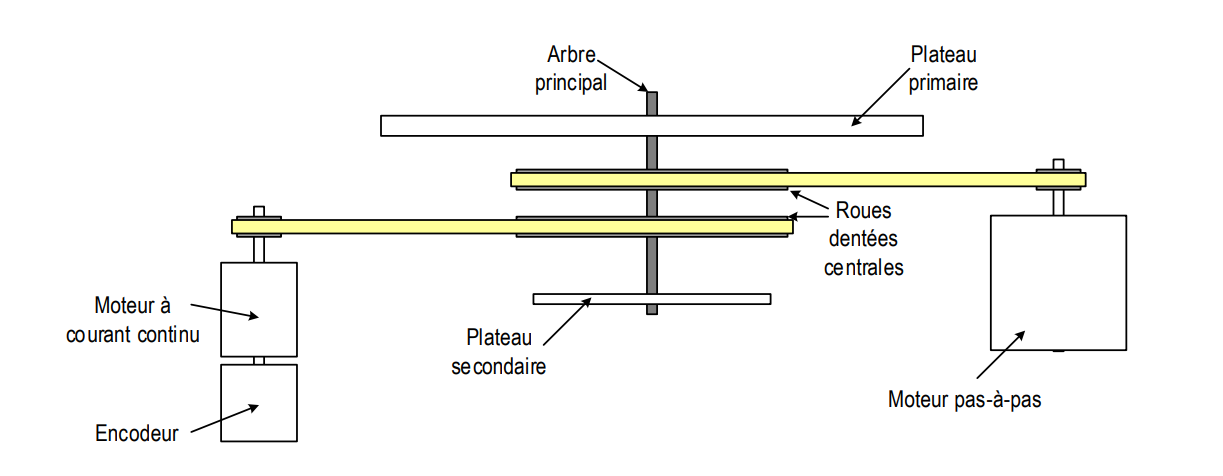
\includegraphics[width=1\linewidth]{Images/Systeme.png}
    \caption{Schéma de la maquette utilisée}
    \label{fig:systeme}
\end{figure}
